% das Papierformat zuerst
\documentclass[a4paper, 11pt]{article}

% deutsche Silbentrennung
\usepackage[ngerman]{babel}

% wegen deutschen Umlauten
\usepackage[utf8]{inputenc}

% Grafikpaket laden
\usepackage{graphicx}

% hier beginnt das Dokument
\begin{document}

% das Abbildungsverzeichnis
\listoffigures

% Grafik auf neuer Seite anzeigen
\newpage

Jetzt soll eine Grafik angezeigt werden. Dabei werden wir feststellen, dass die
Grafik über diesem Satz angezeigt wird, obwohl wir den Befehl für die Grafik
erst in den nächsten Zeilen geben.
\begin{figure}
	\centering
	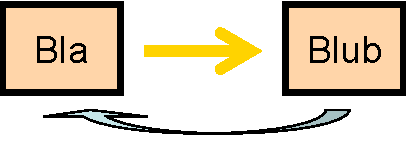
\includegraphics{grafik.pdf}
	\caption{eine Grafik ohne Sinn und Verstand}
	\label{img:grafik-dummy}
\end{figure}

% eine weitere Seite
\newpage

Weiterhin wollen wir an dieser Stelle Bezug auf die Grafik
\ref{img:grafik-dummy} auf Seite \pageref{img:grafik-dummy} nehmen, was uns
hiermit gelungen sein dürfte. Latex passt die Seitenzahl aber auch die Nummer
der Grafik automatisch an, wir müssen uns um nichts kümmern.

Bis jetzt wurde es noch nicht erwähnt, aber man fügt einen neuen Absatz im Text
ein, indem man eine Leerzeile lässt, wie hier gerade gezeigt wurde.

% das ist wohl jetzt das Ende des Dokumentes
\end{document}
